\section{Data Processing}

Before concluding anything from the data, it is first analysed to check if the made assumptions are valid. The assumptions include a stationary channel, uncorrelated samples and finally that the data is Rayleigh distributed.

\subsection{Raw data}

In total 4.184.460 samples have been collected, the values are represented in \autoref{fig:rawFadingMeas}.

\begin{figure}[H]
\centering
\includegraphics[height = \textwidth, angle = -90]{figures/rawFadingMeas.pdf}
\caption{The measured samples spaced in frequency and space.}
\label{fig:rawFadingMeas}
\end{figure}


\subsection{Stationarity}
To see if the channel is stationary it has to be checked in both the frequency domain and the spatial domain. The first step in doing this is to average across the other domain. The result of this can be seen in \autoref{fig:meanFading}. 


\begin{figure}[H]
\centering
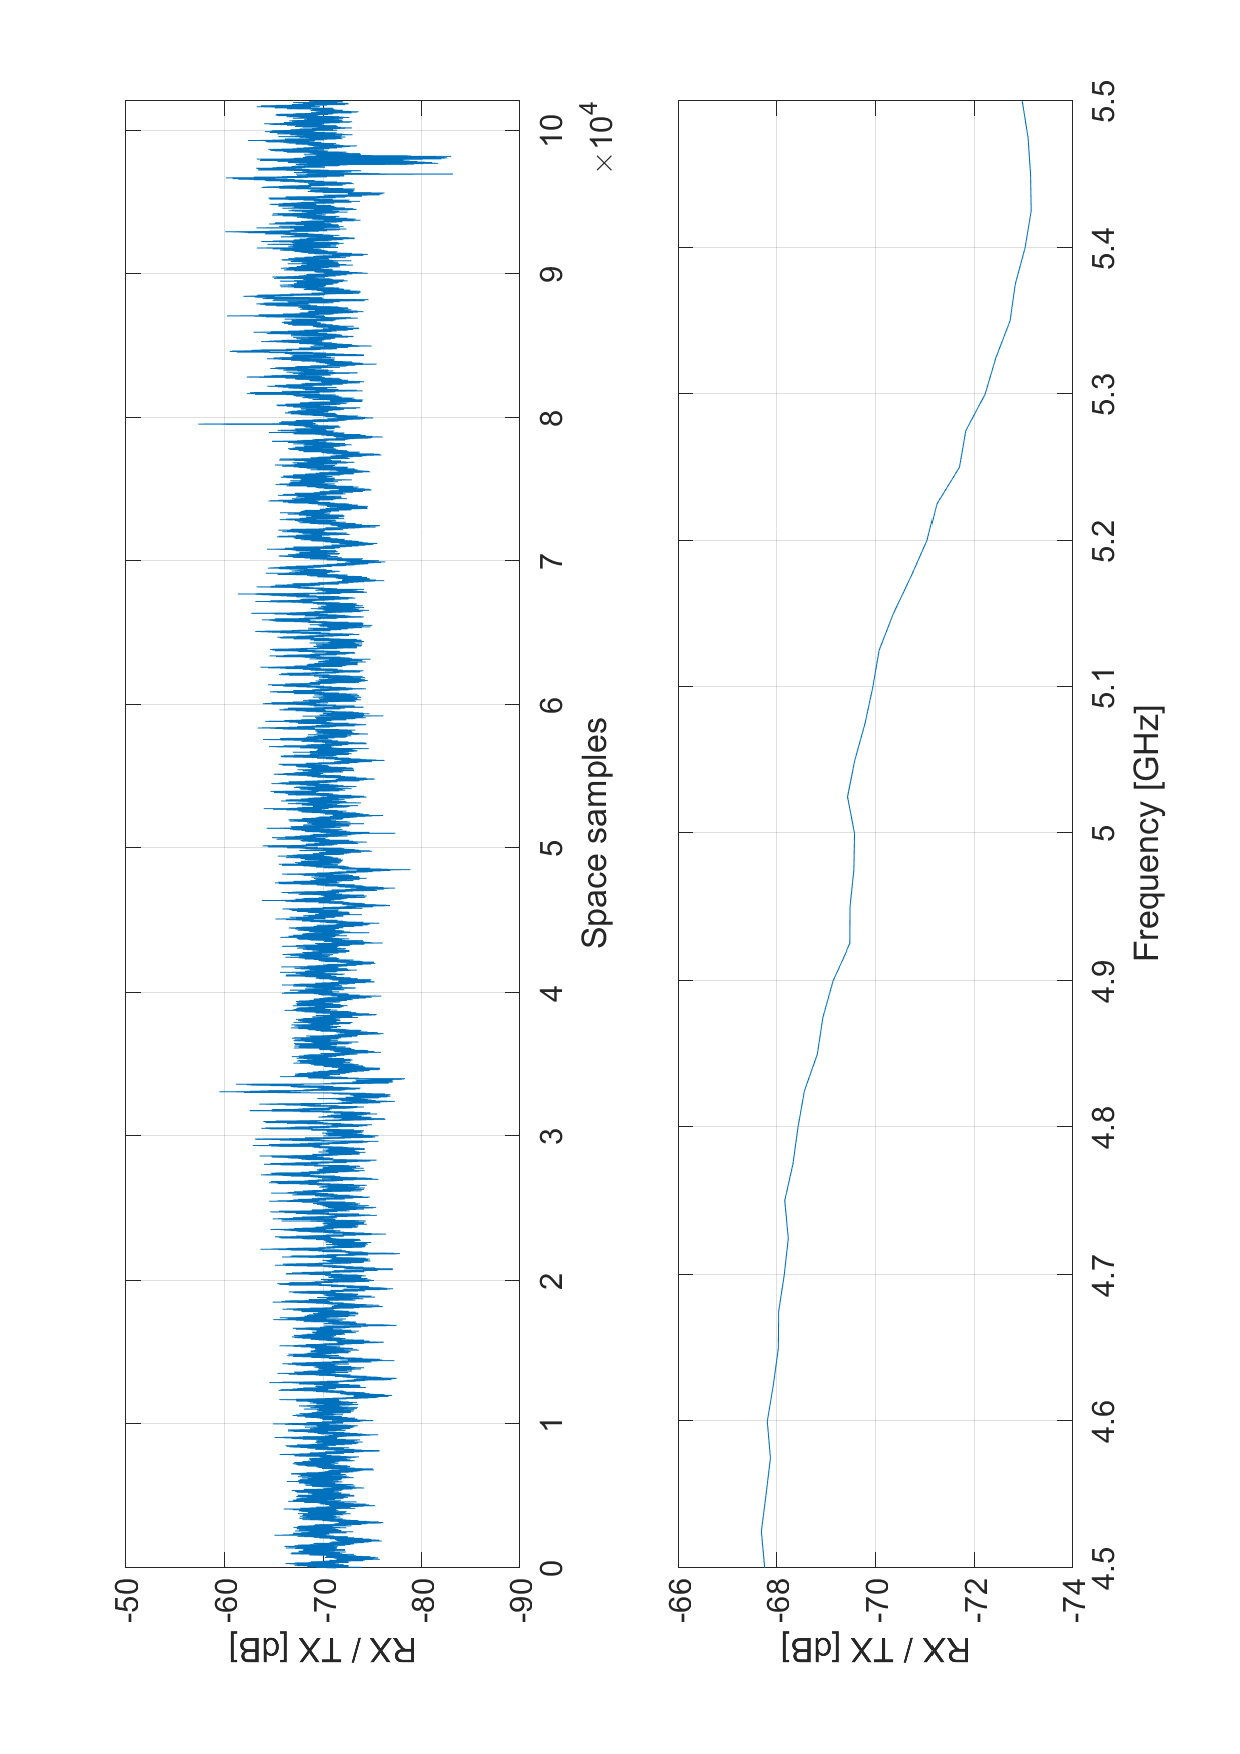
\includegraphics[height = \textwidth, angle = -90]{figures/meanFading.pdf}
\caption{Average values across the frequency and space domain respectively.}
\label{fig:meanFading}
\end{figure}


Note the reason for the spuriousness in the spatial domain has to do with the average being taken only over the 41 frequency samples at each position, where the the more smooth line in the frequency domain is an average across 102.060 samples in space. It can however be seen directly that the power level seems more or less constant across all spatial points, where it drops with frequency. This is expected as the \gls{PL} is dependent on the wavelength.  

A condition that has to be met is that no dominant componet is present, to check this all samples are normalized with regards to the mean values seen in \autoref{fig:meanFading}, the normalize data is then fitted to a Rician distribution and the non-centrality parameter is found using matlabs \textit{fitdist} function as can be seen in \autoref{lst:a_value}. 

\lstset{caption={Code implementation of the a value calculation.}, label=lst:a_value}
\begin{lstlisting}
% The measured values is stored in data which is a 41x102060 matrix with
% the rows being frequency samples and the coloums being space samples

PL = repmat(mean(data,2),1,102060);   % Determine PL by averaging across space dimension 
dataN = data./PL;                     % Normalize data wrt. frequency
dataS = reshape(dataN,41*102060,1);   % Reshape to vector format

pd = fitdist(dataS,'Rician');         % Fit data to a Rician distribution
pd.s                                  % Show non-centrality parameter for space domain

PL = repmat(mean(data,1),41,1);       % Determine PL by averaging across frequency dimension
dataN = data./PL;                     % Normalize data wrt. space
dataF = reshape(dataN,41*102060,1);   % Reshape to vector format

pd = fitdist(dataF,'Rician');         % Fit data to a Rician distribution
pd.s                                  % Show non-centrality parameter for frequency domain
\end{lstlisting}

From this it can be found that the non-centrality parameter of the two domains are 0.0267 and 0.0319 for space and frequency domain respectively. That means that any dominant component is negligible compared to the random components, and it can therefore by concluded that the channel behaves stationary.

%\begin{figure}
%\input{figures/Norm_sapce_3.tex}
%\end{figure}
%\begin{figure}
%\input{figures/Not_Norm_sapce.tex}
%\end{figure}